\begin{figure}
\centering
  \begin{tabular}{c}
  
%%%%% expt1  
  
  \begin{subfigure}{0.45\textwidth}
 \tabl{c}{\scalebox{0.8}{\begin{tikzpicture}
      \begin{axis}[
	xlabel={timestep},
	ylabel={Cumulative regret},
       clip mode=individual,grid,grid style={gray!30},
  legend style={at={(0.5,-0.2)},anchor=north,legend columns=3} ]  
  % UCB    

\addplot table[x index=0,y index=1,col sep=tab,each nth point={10}] {results/Expt1/UCB_Vcomp_subsampled.txt};
\addplot table[x index=0,y index=1,col sep=tab,each nth point={10}] {results/Expt1/DMEDcomp_subsampled.txt};
\addplot table[x index=0,y index=1,col sep=tab,each nth point={10}] {results/Expt1/KLUCBcomp_subsampled.txt};
\addplot table[x index=0,y index=1,col sep=tab,each nth point={10}] {results/Expt1/MOSScomp_subsampled.txt};
\addplot table[x index=0,y index=1,col sep=tab,each nth point={10}] {results/Expt1/UCB1comp_subsampled.txt};
\addplot table[x index=0,y index=1,col sep=tab,each nth point={10}] {results/Expt1/TScomp_subsampled.txt};
\addplot table[x index=0,y index=1,col sep=tab,each nth point={10}] {results/Expt1/clUCBcomp_subsampled.txt};
      \legend{UCB-V,DMED,KL-UCB,MOSS,UCB1,TS,ClusUCB(p=4)}
      \end{axis}
      \end{tikzpicture}}\\}
			\caption{Experiment $1$: $20$ Bernoulli-distributed arms with $r_{i_{a_{i}\neq a^{*}}}=0.07$ and $r^{*}=0.1$.}
  \label{fig:1}
  \end{subfigure}
	\\
	%%%%%%% Expt 2
	  \begin{subfigure}{0.45\textwidth}
 \tabl{c}{\scalebox{0.8}{\begin{tikzpicture}
      \begin{axis}[
	xlabel={timestep},
	ylabel={Cumulative regret},
       clip mode=individual,grid,grid style={gray!30},
  legend style={at={(0.5,-0.2)},anchor=north,legend columns=3} ]
      % UCB
\addplot table[x index=0,y index=1,col sep=tab,each nth point={10}] {results/Expt2/clUCBCcomp_subsampled.txt};
\addplot table[x index=0,y index=1,col sep=tab,each nth point={10}] {results/Expt2/clUCBNCcomp_subsampled.txt};
\addplot table[x index=0,y index=1,col sep=tab,each nth point={10}] {results/Expt2/Med_Elimcomp_subsampled.txt};
\addplot table[x index=0,y index=1,col sep=tab,each nth point={10}] {results/Expt2/UCB_Improvedcomp_subsampled.txt};
\addplot table[x index=0,y index=1,col sep=tab,each nth point={10}] {results/Expt2/MOSScomp_subsampled.txt};
\addplot table[x index=0,y index=1,col sep=tab,each nth point={10}] {results/Expt2/UCB1comp_subsampled.txt};
      \legend{ClusUCB(p=20), ClusUCB-AE(p=1), Med-Elim,UCB-Improved,MOSS,UCB1}
      \end{axis}
      \end{tikzpicture}}\\}
			\caption{Experiment $2$: $100$ Gaussian-distributed arms with $r_{i_{a_{i}\neq a^{*}:1-33}}=0.01$, $r_{i_{a_{i}\neq a^{*}:34-99}}=0.06$ and $r^{*}_{i=100}=0.1$.}
  \label{fig:2}
  \end{subfigure}
	%\\
  \end{tabular}
\caption{Cumulative regret for various bandit algorithms on three stochastic K-armed bandit environments. 
}
\label{fig:karmed}
\end{figure}



%\begin{figure}[!tbp]
%\label{fig:1}
%\begin{minipage}[b]{0.5\textwidth}
%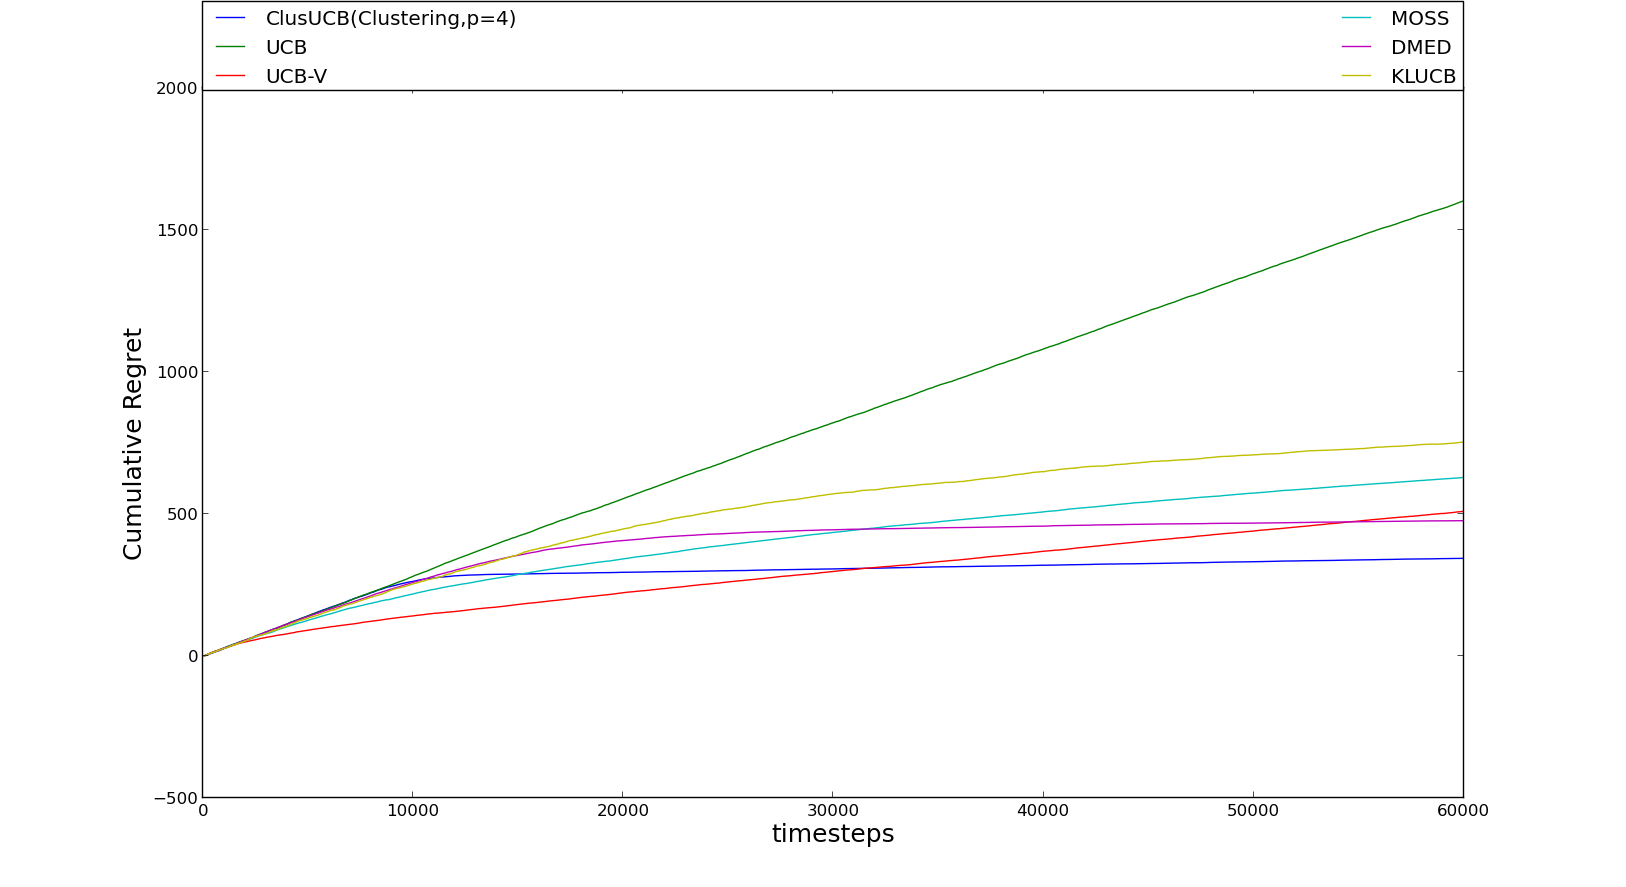
\includegraphics[width=\textwidth]{img/ClusUCB_variousAlgo.png}
%
%\caption{Experiment 1: Regret for various Algorithms. $T=60000$}
%\end{minipage}
%\end{figure}
%
%\hspace{0.1em}
%
%\begin{figure}[!tbp]
%\label{fig:2}
%\begin{minipage}[b]{0.5\textwidth}
%
%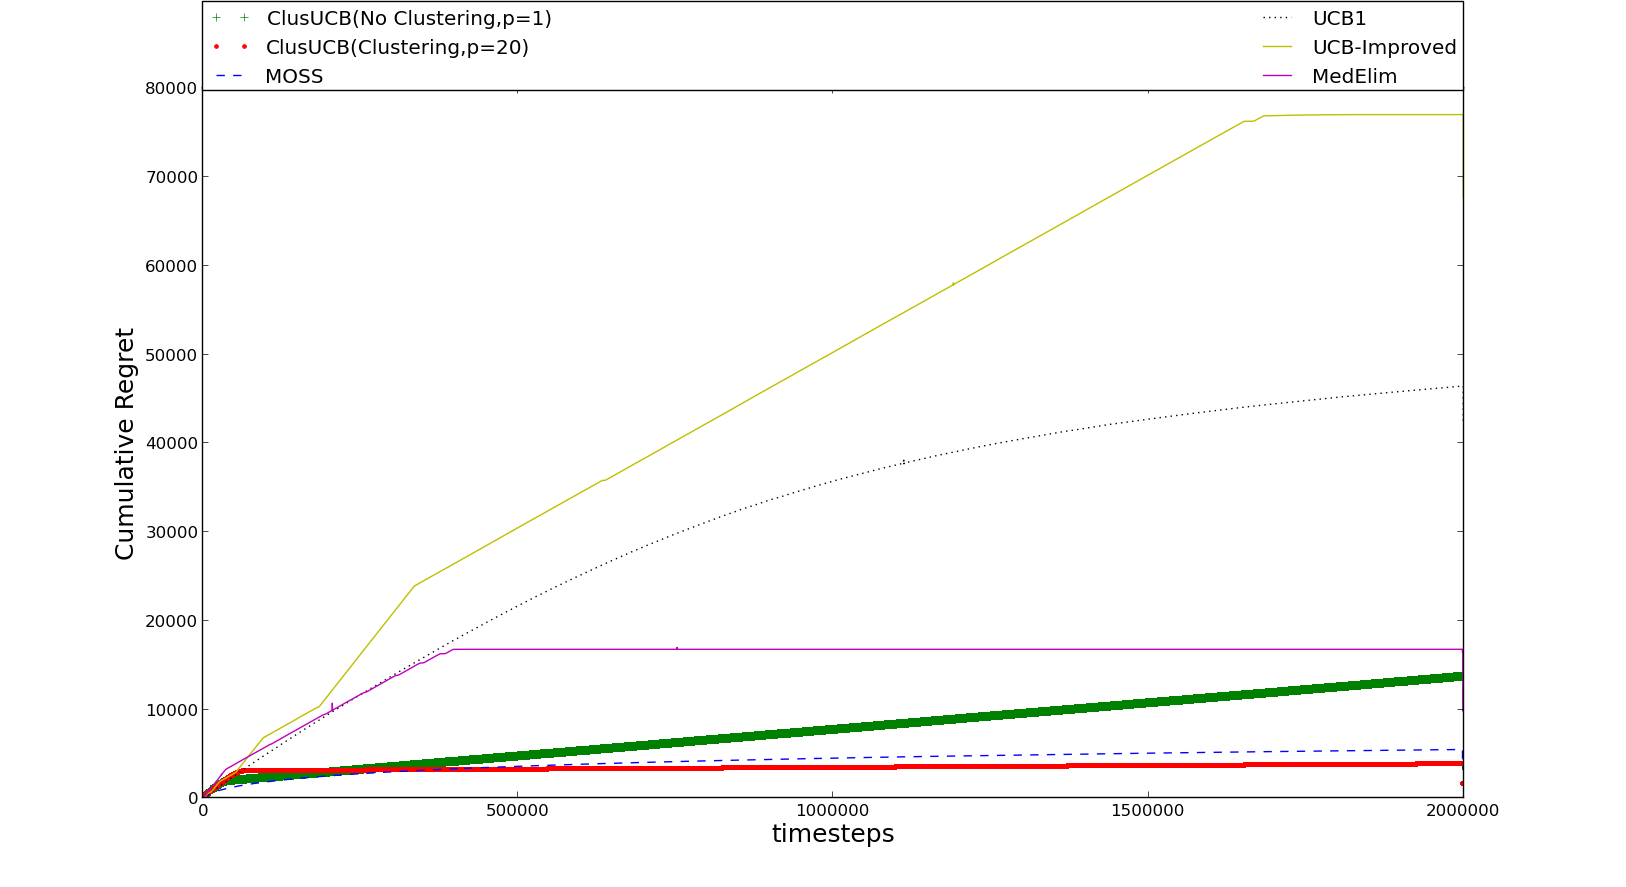
\includegraphics[width=\textwidth]{img/clusUCB_variousAlgo(expt2)_Final.png}
%\caption{Experiment 2: Regret for various Algorithms. $T=2\times 10^{6}$}
%\end{minipage}
%\end{figure}
%
%\hspace{0.1em}
%
%\begin{figure}[!tbp]
%\label{fig:3}
%\begin{minipage}[b]{0.5\textwidth}
%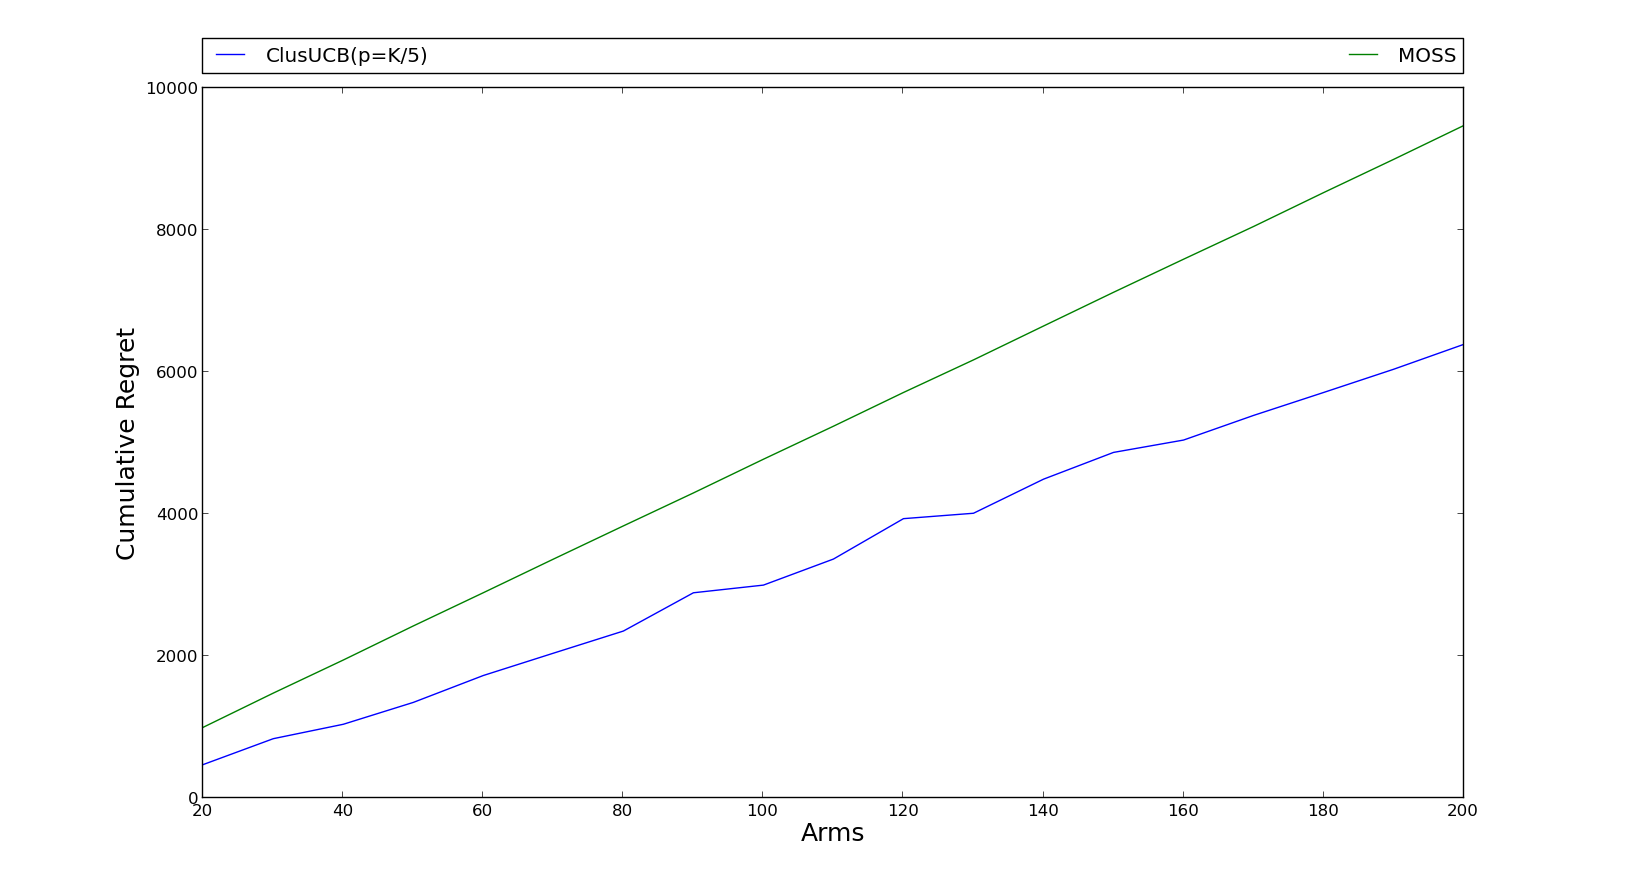
\includegraphics[width=\textwidth]{img/clUCB_MOSS_expt3.png}
%\caption{Experiment 3: Regret Growth for ClusUCB and MOSS . $T=10^{5} + K^{2}\times 10^{4}$ for $K=20$ to $200$}
%\end{minipage}
%\end{figure}
%
%\hspace{0.1em}
%


%In the stochastic bandit literature there are several powerful algorithms with and without proven regret bounds. Algorithms like $\epsilon$-greedy(\cite{sutton1998reinforcement}) or softmax(\cite{sutton1998reinforcement}) or UCB-Tuned(\cite{auer2002finite}) has no proven regret bounds. Again algorithms like UCB-$\delta$(\cite{abbasi2011improved}) with proven regret bound better than UCB1  falls within the realm of fixed confidence setting whereas one has to provide the probability of error $\delta$. We also make a distinction between frequentist based approach like the UCB algorithms and the Bayesian approach like the Thompson Sampling(\cite{agrawal2011analysis}). 
For the sake of performance comparison using cumulative regret as the metric, we implement the following algorithms:  KL-UCB\cite{garivier2011kl}, DMED\cite{honda2010asymptotically}, MOSS\cite{audibert2009minimax}, UCB1\cite{auer2002finite}, UCB-Improved\cite{auer2010ucb}, Median Elimination\cite{even2006action}, Thompson Sampling(TS)\cite{agrawal2011analysis} and UCB-V\cite{audibert2009exploration}\footnote{The implementation for KL-UCB and DMED are taken from \cite{CapGarKau12}}. For parameter settings of ClusUCB and further experiments see Appendix \ref{App:Further:Expt}.

The first experiment is conducted over a testbed of $20$ arms for the test-cases involving Bernoulli reward distribution with expected rewards of the arms $r_{i_{a_{i}\neq a^{*}}}=0.07$ and $r^{*}=0.1$. These type of cases are frequently encountered in web-advertising domain. The horizon $T$ is set to $60000$ and the number of clusters $p$ for ClusUCB is set to $4$. The regret is averaged over $100$ independent runs and is shown in Figure \ref{fig:1}. 
ClusUCB, MOSS, UCB1, UCB-V, KL-UCB, TS and DMED are run in this experimental setup and we observe that ClusUCB performs better than all the aforementioned algorithms. Because of the short horizon $T$, we do not implement UCB-Improved and Median Elimination on this test-case. We also see that in this case the cumulative regret of ClusUCB and TS are very close to each other though ClusUCB is slightly better.
The second experiment is conducted over a testbed of $100$ arms involving Gaussian reward distribution with expected rewards of the arms $r_{i_{a_{i}\neq a^{*}:1-33}}=0.01$, $r_{i_{a_{i}\neq a^{*}:34-99}}=0.06$ and $r^{*}_{i=100}=0.1$ with variance set at $\sigma = 0.3,\forall i\in A$. The horizon $T$ is set for a large duration of $2\times 10^{6}$ and the number of clusters $p=20$. The regret is averaged over $100$ independent runs and is shown in Figure \ref{fig:2}. In this case, in addition to ClusUCB, we also show the performance of no-clustering version of ClusUCB algorithm (i.e., $p=1$).   From the results sin Figure \ref{fig:2}, we observe that ClusUCB with $p=20$ outperforms ClusUCB with $p=1$ as well as MOSS, UCB1, UCB-Improved and Median-Elimination($\epsilon=0.03,\delta=0.1$). We also observed that the ClusUCB variant that uses only  the arm elimination condition in Algorithm \ref{alg:clusucb} performs worse than the variant that employs both cluster and arm elimination conditions. Also UCB-Improved performs the worst and it confirms our assumption that it spends too much pulls in initial exploration.

%We also see that in this testbed UCB-Improved performs the worst and it confirms our assumption that it spends too much pulls in the initial exploration.

%We set $\psi=1$, $\rho_{s}=\frac{1}{2^{m+1}}$ and $\rho_{a}=\frac{1}{2^{2m+1}}$.

%The jumps in the graph for ClusUCB happens because of the error(eliminating optimal arm) and the margin of error(in red) is also shown in the graph. 
%\todos{I did not see this jump in the txt files shared for Expt 3}
